% ---------------------------------------------------------------------------
%  Galeria de componentes -- tema usach v2.1
%  Catalogo para copiar y pegar. Compilar:
%    latexmk -pdf -outdir=build galeria.tex
%  La opcion xcolor=table habilita \rowcolors sin choque de opciones.
% ---------------------------------------------------------------------------
\documentclass[11pt,aspectratio=169,xcolor=table]{beamer}

\IfFileExists{spanish.ldf}{%
  \usepackage[spanish,es-noquoting,es-nodecimaldot]{babel}%
}{%
  \usepackage[T1]{fontenc}
  \renewcommand{\figurename}{Figura}
  \renewcommand{\tablename}{Tabla}
}
\usepackage[utf8]{inputenc}
\usepackage{amsmath,amssymb}
\usepackage{booktabs,tabularx,multirow}
\usepackage{pgfplots}
\usepackage{listings}
\usepackage[ruled,vlined,linesnumbered,spanish]{algorithm2e}
\SetKw{KwSeguir}{seguir}
\usetikzlibrary{positioning,arrows.meta,shapes.geometric}
\usepackage{microtype}

\usetheme[pei]{usach}   % 'pei' habilita la paleta PEI 2030 en los graficos

\title[Galería de componentes]{Galería de componentes}
\subtitle{Todo lo que el tema sabe componer, listo para copiar}
\author{Iván Ahumada}
\date{Septiembre de 2026}
\usachfacultad{Facultad de Ingeniería}
\usachdepartamento{Departamento de Ingeniería Informática}
\usachprograma{Magíster en Ingeniería Informática}
\usachasignatura{Plantilla institucional}
\usachprofesor{---}
\institute[USACH]{Universidad de Santiago de Chile}

\begin{document}

\usachportada

\begin{frame}{Contenido}
  \tableofcontents
\end{frame}

% ===========================================================================
\section{Texto y estructura}
% ===========================================================================

\begin{frame}{Listas}{Tres niveles, con y sin aire adicional}
  \begin{columns}[T,onlytextwidth]
    \begin{column}{0.48\textwidth}
      Lista compacta, por defecto:
      \begin{itemize}
        \item Lectura acumulada por predio.
        \item Consumo del período.
          \begin{itemize}
            \item Diferencia de lecturas consecutivas.
            \item Corrección por días facturados.
              \begin{itemize}
                \item Calendario comercial.
              \end{itemize}
          \end{itemize}
      \end{itemize}
    \end{column}
    \begin{column}{0.48\textwidth}
      Con \texttt{\textbackslash usachaire}, para láminas de pocos puntos:
      \begin{itemize}\usachaire
        \item El umbral se calibra por tipo de cliente.
        \item El modelo corre sin conexión.
        \item La corrección ocurre en la misma visita.
      \end{itemize}

      \begin{description}
        \item[MAD] Desviación absoluta mediana.
        \item[VarPro] Separación de variables lineales.
      \end{description}
    \end{column}
  \end{columns}
\end{frame}

\begin{frame}{Énfasis, citas y notas}
  El texto normal va en gris institucional. Se puede \alert{destacar con el rojo
  oficial}, marcar \textbf{peso} o \emph{matiz}, y anotar al pie\footnote{Las
  notas al pie usan el mismo gris que los metadatos.} sin romper el ritmo.

  \usachcita{La calidad del dato se define en el punto de captura, no en el
  escritorio.}{Cuadrilla norte, bitácora de terreno, marzo de 2026}

  \begin{itemize}
    \item Enlaces: \url{https://guiaweb.usach.cl}
    \item Referencia cruzada al Cuadro~\ref{tab:comparacion}.
  \end{itemize}
\end{frame}

\begin{frame}{Aparición progresiva}
  \begin{itemize}\usachaire
    \item<1-> El residuo se calcula con la ventana móvil de doce períodos.
    \item<2-> Si supera el umbral, la lectura se marca en el dispositivo.
    \item<3-> El lector confirma o corrige antes de cerrar la visita.
  \end{itemize}
  \onslide<3->{%
    \begin{block}{Efecto}
      El ciclo de facturación no se vuelve a abrir.
    \end{block}}
\end{frame}

% ===========================================================================
\section{Bloques y cifras}
% ===========================================================================

\begin{frame}{Los tres bloques}
  \begin{columns}[T,onlytextwidth]
    \begin{column}{0.48\textwidth}
      \begin{block}{Definición}
        Una lectura es anómala si su residuo robusto supera tres desviaciones.
      \end{block}
      \begin{exampleblock}{Caso favorable}
        Predio residencial con consumo estable: el umbral no genera falsos
        positivos en 24 meses.
      \end{exampleblock}
    \end{column}
    \begin{column}{0.48\textwidth}
      \begin{alertblock}{Restricción}
        El modelo corre en el dispositivo del lector, sin conexión garantizada.
      \end{alertblock}
      \begin{block}{Bloque con lista}
        \begin{itemize}
          \item Ventana: 12 períodos.
          \item Umbral: $|r_t| > 3$.
        \end{itemize}
      \end{block}
    \end{column}
  \end{columns}
\end{frame}

\begin{frame}{Cifras destacadas}{Una fila de tres o cuatro, no más}
  \usachdatos{%
    \begin{minipage}[t]{0.23\linewidth}\usachdato{8\,\%}{lecturas fuera de rango}\end{minipage}\hfill
    \begin{minipage}[t]{0.23\linewidth}\usachdato{14 días}{demora media de detección}\end{minipage}\hfill
    \begin{minipage}[t]{0.23\linewidth}\usachdato{1,7}{revisitas por corrección}\end{minipage}\hfill
    \begin{minipage}[t]{0.23\linewidth}\usachdato{40 kB}{tamaño del modelo}\end{minipage}}

  \vfill
  Debajo de la fila conviene una sola frase que explique de dónde salen los
  números, no una segunda lista.
  \usachfuente{base de lecturas 2024--2026, 1,2 millones de registros.}
\end{frame}

\usachdestacado{Si el dato se corrige en terreno, el ciclo de facturación no
se vuelve a abrir.}

% ===========================================================================
\section{Tablas}
% ===========================================================================

\begin{frame}{Tabla de resultados}{\texttt{booktabs}: sin líneas verticales}
  \begin{table}
    \centering\small
    \begin{tabular}{@{}lrrr@{}}
      \toprule
      Estrategia & Precisión & Recall & Latencia \\
      \midrule
      Rango fijo por tarifa      & 0,41 & 0,88 & inmediata \\
      Residuo robusto (MAD)      & 0,79 & 0,84 & inmediata \\
      \textbf{Modelo estacional} & \textbf{0,86} & \textbf{0,81} & 2 s \\
      \bottomrule
    \end{tabular}
    \caption{Desempeño sobre 24 meses de lecturas etiquetadas.}
    \label{tab:comparacion}
  \end{table}
  \usachfuente{elaboración propia.}
\end{frame}

\begin{frame}{Tabla ancha con filas alternadas}
  \rowcolors{2}{usachgris10}{white}
  \begin{table}
    \centering\footnotesize
    \begin{tabularx}{\textwidth}{@{}lXrr@{}}
      \toprule
      \rowcolor{usachgris}
      \usachcab{Sector} & \usachcab{Descripción} &
      \usachcab{Lecturas} & \usachcab{Marcadas} \\
      \midrule
      Norte    & Residencial denso, medidores 2019--2022 & 184\,220 & 12\,410 \\
      Centro   & Mixto comercial, medidores mixtos       & 156\,880 &  9\,004 \\
      Sur      & Residencial disperso, red antigua       & 121\,340 & 14\,988 \\
      Poniente & Industrial, macromedición               &  38\,110 &  1\,206 \\
      \bottomrule
    \end{tabularx}
    \caption{Distribución de lecturas por sector operativo.}
  \end{table}
  \usachfuente{sistema comercial, corte al 31 de agosto de 2026.}
\end{frame}

% ===========================================================================
\section{Gráficos}
% ===========================================================================

\begin{frame}{Serie de tiempo}{Estilo \texttt{usach} de \texttt{pgfplots}}
  \centering
  \begin{tikzpicture}
    \begin{axis}[usach, width=0.86\textwidth, height=0.52\textheight,
      xlabel={Mes}, ylabel={Lecturas marcadas},
      xmin=1, xmax=12, ymin=0, ymax=1800,
      xtick={1,3,5,7,9,11}, ymajorgrids,
      legend style={at={(0.5,1.04)},anchor=south,legend columns=-1}]
      \addplot coordinates {(1,1620)(2,1580)(3,1490)(4,1440)(5,1310)(6,1180)
                            (7,1120)(8,980)(9,910)(10,860)(11,820)(12,790)};
      \addlegendentry{Con validación en terreno}
      \addplot coordinates {(1,1650)(2,1610)(3,1640)(4,1590)(5,1620)(6,1570)
                            (7,1600)(8,1560)(9,1580)(10,1540)(11,1570)(12,1530)};
      \addlegendentry{Línea base}
    \end{axis}
  \end{tikzpicture}
  \usachfuente{elaboración propia a partir del sistema comercial.}
\end{frame}

\begin{frame}{Barras y dispersión}
  \begin{columns}[T,onlytextwidth]
    \begin{column}{0.49\textwidth}
      \centering
      \begin{tikzpicture}
        \begin{axis}[usach, width=\textwidth, height=0.42\textheight,
          ybar, bar width=8pt, ymin=0, ymax=1, cycle list name=usachciclobarras,
          symbolic x coords={Rango,MAD,Estacional},
          xtick=data, ylabel={Métrica}, ymajorgrids,
          legend style={at={(0.5,1.04)},anchor=south,legend columns=-1}]
          \addplot coordinates {(Rango,0.41)(MAD,0.79)(Estacional,0.86)};
          \addlegendentry{Precisión}
          \addplot coordinates {(Rango,0.88)(MAD,0.84)(Estacional,0.81)};
          \addlegendentry{Recall}
        \end{axis}
      \end{tikzpicture}
    \end{column}
    \begin{column}{0.49\textwidth}
      \centering
      \begin{tikzpicture}
        \begin{axis}[usach, width=\textwidth, height=0.42\textheight,
          only marks, mark size=1.3pt,
          xlabel={Consumo previo (m$^3$)}, ylabel={Residuo $r_t$},
          ymajorgrids]
          \addplot+[mark=*] coordinates
            {(4,0.3)(7,-0.6)(9,0.9)(12,0.1)(15,-1.1)(18,0.4)(21,-0.2)(25,1.2)
             (28,-0.8)(31,0.6)(35,-0.3)(38,1.0)};
          \addplot+[mark=triangle*] coordinates
            {(6,3.8)(14,-4.2)(23,3.4)(33,4.9)};
        \end{axis}
      \end{tikzpicture}
    \end{column}
  \end{columns}
  \vskip0.3em
  Con la opción \texttt{pei} el ciclo de colores usa la paleta PEI 2030; sin
  ella, rojo y grises institucionales.
\end{frame}

% ===========================================================================
\section{Algoritmos y código}
% ===========================================================================

\begin{frame}{Pseudocódigo}{\texttt{algorithm2e}}
  \begin{algorithm}[H]
    \footnotesize
    \KwIn{Serie de lecturas $y_1,\dots,y_n$; umbral $\tau$; ventana $w$}
    \KwOut{Conjunto $A$ de lecturas marcadas}
    $A \leftarrow \emptyset$\;
    \For{$t \leftarrow w+1$ \KwTo $n$}{
      $\Delta \leftarrow \{y_i - y_{i-1} : t-w \le i < t\}$\;
      $m \leftarrow \operatorname{med}(\Delta)$\;
      $s \leftarrow 1{,}4826 \cdot \operatorname{MAD}(\Delta)$\;
      \lIf{$s = 0$}{\KwSeguir \tcp*[f]{predio sin variación}}
      $r_t \leftarrow (y_t - y_{t-1} - m)/s$\;
      \If{$|r_t| > \tau$}{
        $A \leftarrow A \cup \{t\}$ \tcp*{marcar en el dispositivo}
      }
    }
    \Return{$A$}\;
    \caption{Detección de lecturas anómalas por residuo robusto}
  \end{algorithm}
\end{frame}

\begin{frame}[fragile]{Código fuente}{\texttt{listings} con estilo \texttt{usach}}
\begin{lstlisting}[language=Python]
import numpy as np

def residuo_robusto(lecturas, ventana=12):
    """Residuo estandarizado por MAD sobre el consumo del periodo."""
    consumo = np.diff(lecturas)
    m = np.median(consumo[-ventana:])
    s = 1.4826 * np.median(np.abs(consumo[-ventana:] - m))
    if s == 0:            # predio sin variacion
        return 0.0
    return (consumo[-1] - m) / s
\end{lstlisting}
  Las láminas con \texttt{lstlisting} necesitan la opción \texttt{[fragile]}.
\end{frame}

\begin{frame}{Ecuaciones}{Matemática serif sobre texto sans, como en un paper}
  La ecuación que sostiene el argumento va en panel:

  \begin{usachformula}
    \[
      r_t \;=\; \frac{\Delta y_t - \operatorname{med}(\Delta y)}
                     {1{,}4826 \cdot \operatorname{MAD}(\Delta y)},
      \qquad \Delta y_t = y_t - y_{t-1}.
    \]
  \end{usachformula}

  El resto va en el flujo del texto, sin caja: se marca la lectura cuando
  $|r_t| > \tau$ con $\tau = 3$.
\end{frame}

\begin{frame}{Ecuaciones en el flujo}
  El residuo estandarizado y su umbral:
  \begin{align}
    r_t &= \frac{\Delta y_t - \operatorname{med}(\Delta y)}
                {1{,}4826 \cdot \operatorname{MAD}(\Delta y)}, &
    \Delta y_t &= y_t - y_{t-1}, \\
    A &= \{\, t : |r_t| > \tau \,\}, & \tau &= 3.
  \end{align}

  Con casos:
  \[
    \text{marca}(t) =
    \begin{cases}
      1, & |r_t| > \tau \text{ y } s_t > 0,\\
      0, & \text{en otro caso.}
    \end{cases}
  \]
\end{frame}

% ===========================================================================
\section{Imágenes y diagramas}
% ===========================================================================

\begin{frame}{Figura centrada}
  \begin{figure}
    \centering
    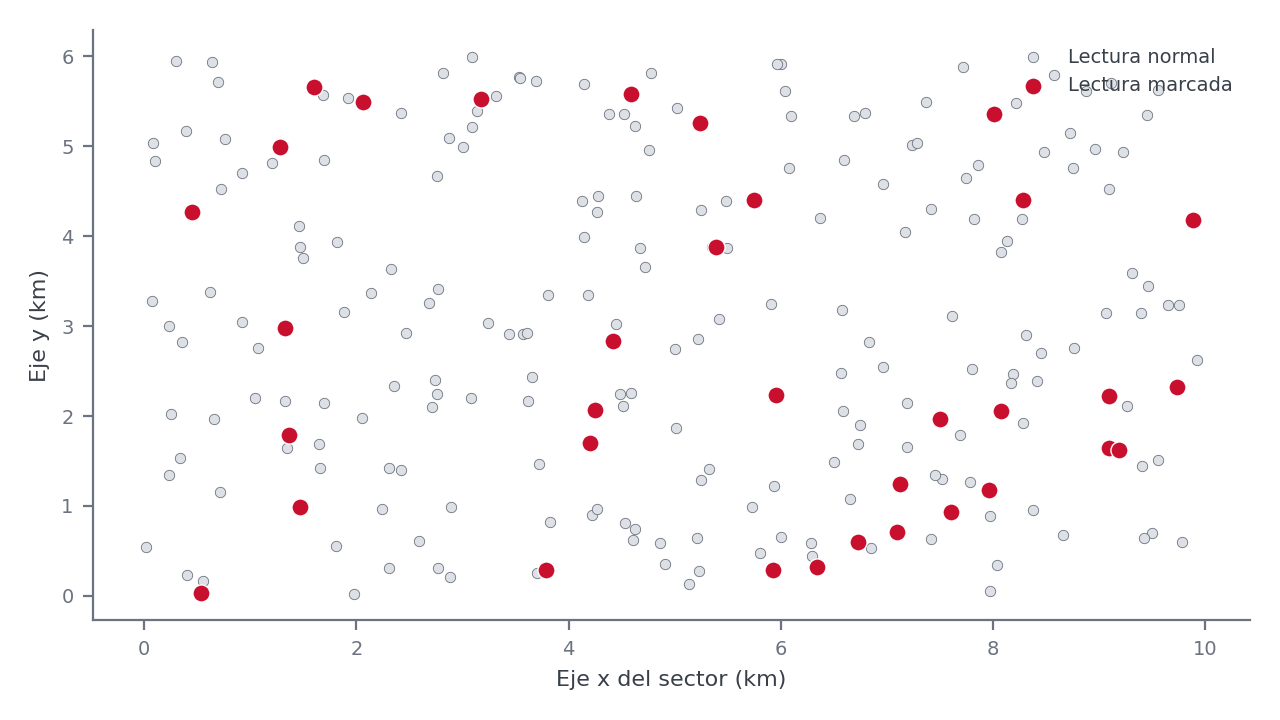
\includegraphics[width=0.60\textwidth]{assets/ejemplo-mapa.png}
    \caption{Distribución espacial de lecturas marcadas en el sector norte.}
  \end{figure}
  \usachfuente{elaboración propia sobre la malla de medidores.}
\end{frame}

\begin{frame}{Imagen y texto}
  \begin{columns}[T,onlytextwidth]
    \begin{column}{0.52\textwidth}
      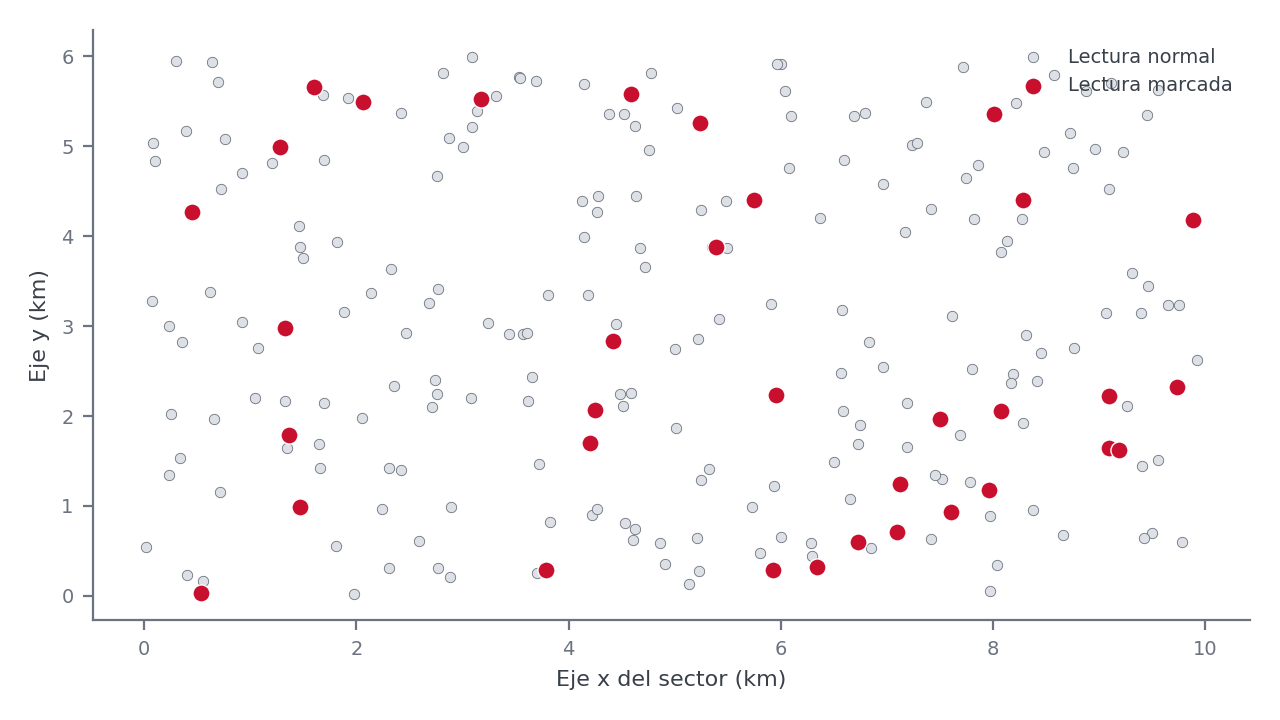
\includegraphics[width=\linewidth]{assets/ejemplo-mapa.png}
      \usachfuente{elaboración propia.}
    \end{column}
    \begin{column}{0.44\textwidth}
      \begin{itemize}\usachaire
        \item Las marcas se concentran en la red antigua.
        \item El sector poniente aporta el 3\,\% de las marcas.
        \item La densidad no explica por sí sola la tasa de anomalías.
      \end{itemize}
    \end{column}
  \end{columns}
\end{frame}

\usachlaminaimagen{assets/ejemplo-fondo.jpg}{La imagen a sangre lleva velo
institucional: el texto blanco conserva contraste sobre cualquier fotografía.}

\begin{frame}{Diagrama de proceso}{TikZ con la paleta institucional}
  \centering
  \begin{tikzpicture}[
    node distance=0.55cm and 0.75cm,
    caja/.style={draw=usachgris20, fill=usachgris10, text=usachtinta,
      minimum height=1.0cm, text width=2.2cm, align=center,
      font=\fontsize{8}{10}\selectfont, inner sep=3pt},
    acento/.style={caja, fill=usachrojo, text=white, draw=usachrojo},
    flecha/.style={-{Stealth[length=4pt]}, draw=usachgris70, line width=0.7pt}]
    \node[caja] (lectura) {Lectura en terreno};
    \node[caja, right=of lectura] (ventana) {Ventana móvil de 12 períodos};
    \node[caja, right=of ventana] (residuo) {Residuo robusto $r_t$};
    \node[acento, right=of residuo] (marca) {Marca y corrección};
    \node[caja, below=1.0cm of residuo] (cierre) {Cierre del ciclo};
    \draw[flecha] (lectura) -- (ventana);
    \draw[flecha] (ventana) -- (residuo);
    \draw[flecha] (residuo) -- node[above, font=\fontsize{7}{8}\selectfont,
      text=usachgris70] {$|r_t|>\tau$} (marca);
    \draw[flecha] (residuo) -- node[right, font=\fontsize{7}{8}\selectfont,
      text=usachgris70] {si no} (cierre);
    \draw[flecha] (marca.south) |- (cierre.east);
  \end{tikzpicture}
  \vskip0.4em
  Cajas grises para los pasos, roja para el único paso que cambia el resultado.
\end{frame}

% ===========================================================================
\section{Cierre}
% ===========================================================================

\begin{frame}[allowframebreaks]{Referencias}
  \begin{thebibliography}{9}
    \bibitem{rousseeuw1993}
      Rousseeuw, P. y Croux, C. (1993).
      \newblock Alternatives to the median absolute deviation.
      \newblock \emph{Journal of the American Statistical Association}, 88(424).
    \bibitem{mng2024}
      Universidad de Santiago de Chile (2024).
      \newblock \emph{Manual de Normas Gráficas 2024-2S}.
  \end{thebibliography}
\end{frame}

\usachcierre{ivan.ahumada@usach.cl \\ Departamento de Ingeniería Informática}

\appendix

\begin{frame}{Anexo: parámetros}
  \begin{table}
    \centering\small
    \begin{tabular}{@{}lll@{}}
      \toprule
      Parámetro & Valor & Origen \\
      \midrule
      Ventana móvil        & 12 períodos & calendario comercial \\
      Factor de coherencia & 1,4826      & normalidad asintótica \\
      Umbral               & 3           & calibración 2025 \\
      \bottomrule
    \end{tabular}
  \end{table}
\end{frame}

\end{document}
